\section{Introduction}\label{sec:intro}

\begin{figure}[t]
\centering
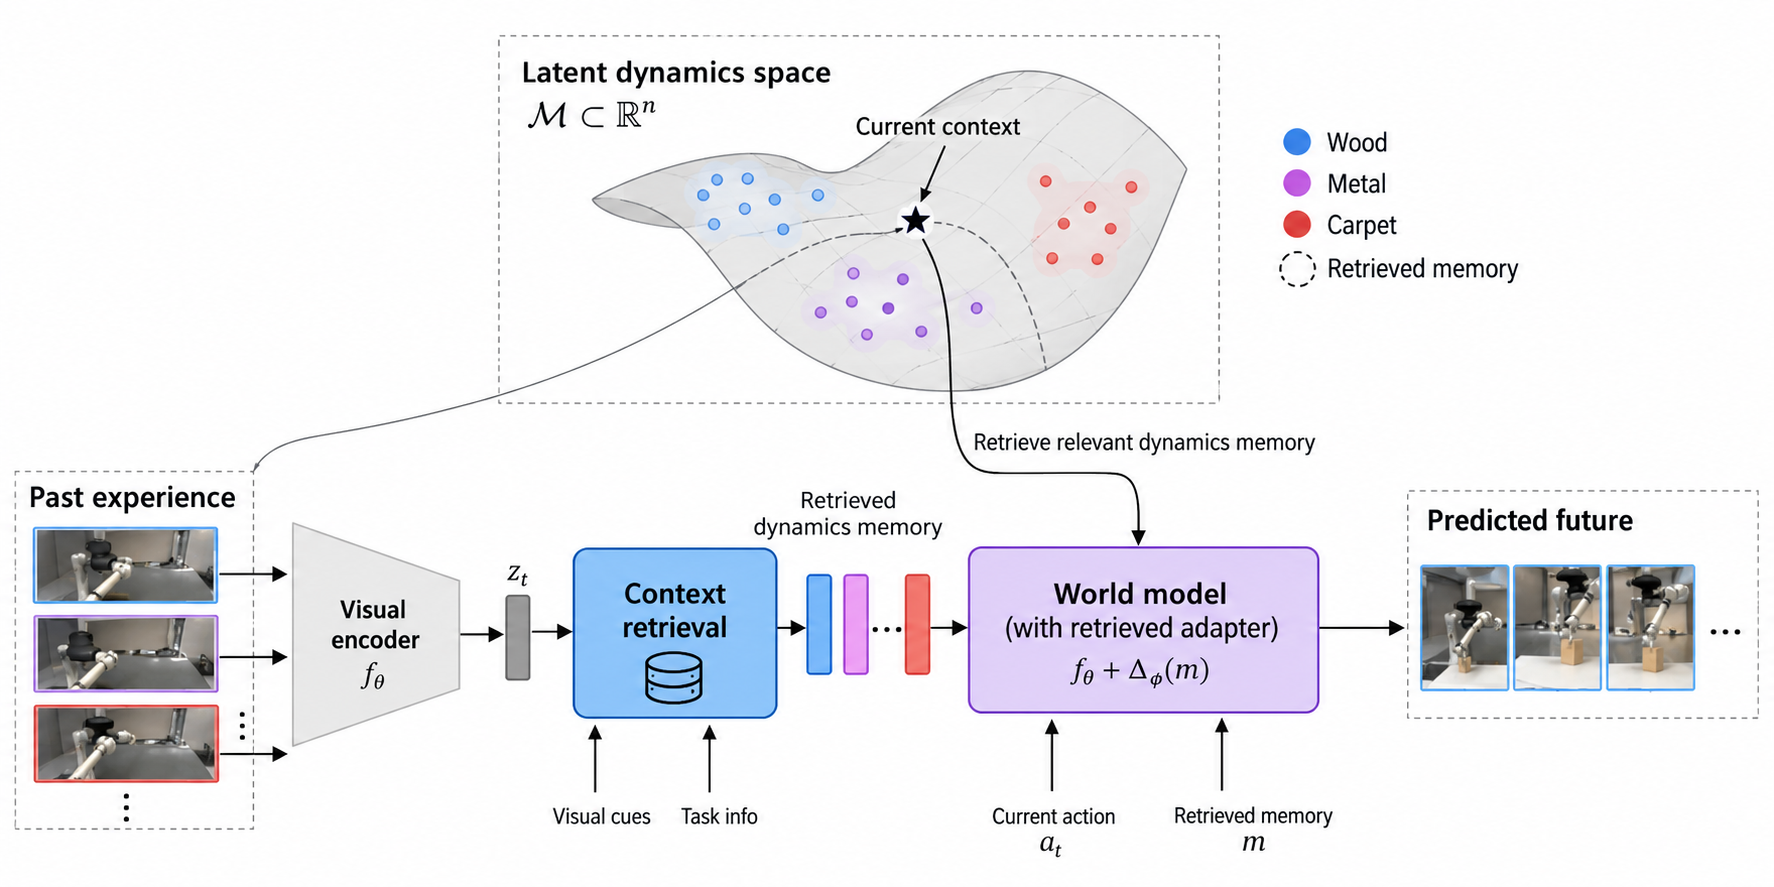
\includegraphics[width=0.92\linewidth]{figures/img/headline.png}
\caption{\textbf{Overview of \method.} A frozen visual world model is augmented with dynamics memories learned during deployment, one per physical context. From visual cues, context retrieval infers which memories apply \emph{before} any interaction, and the retrieved memory corrects the frozen prediction ($f_\theta+\Delta_\phi(m)$ in the figure; $f+\sum_c\pi_e(c)\,m_c$ in \cref{sec:method}).}
\label{fig:headline}
\end{figure}


Visual world models trained on large offline datasets can now plan manipulation tasks directly from images~\citep{zhou2025dinowm,assran2025vjepa2,sobal2025pldm}. Once deployed, however, a robot meets physical conditions its model was never trained on: the same puck slides farther on acrylic than on felt, and a container may be empty or full. A natural remedy is to adapt the model online from its own prediction errors, either by fine-tuning its layers inside the planning loop~\citep{wang2026adajepa} or by training lightweight residual modules around a frozen predictor~\citep{soni2026sandwich}.

This remedy, however, is limited by timing. Consider a robot that must strike a puck so that it stops at a target near a table edge (\cref{fig:teaser}). The correct strike depends on friction and mass, yet the prediction error that would reveal them is observed only after the strike has been executed. Adapting the model at that point improves the next attempt but cannot rescue the current one. Tossing~\citep{zeng2020tossingbot}, the initial force of a lift, and pushing close to an edge share this structure. On such \emph{single-contact tasks}, any scheme driven solely by current-episode errors makes exactly the frozen model's prediction at the moment that matters, however quickly it adapts afterwards (\cref{obs:first}).

Useful information is nevertheless often available before contact, because deployments are repetitive. A robot in a lab or warehouse encounters the same few surfaces, containers and tools many times, and they usually look different from one another. Humans exploit this structure: they maintain separate motor memories for different contexts, recall rather than relearn them when a context returns, and use sensory cues to select the appropriate memory before moving~\citep{heald2021coin,haruno2001mosaic}. This suggests treating adaptation as inference over which known context is active, with learning reserved for new ones.

We instantiate this idea in \method, a module that attaches to any frozen visual world model (\cref{fig:headline}). \method maintains a library of compact Bayesian linear models of the world model's residual error, one per discovered context. Before contact, a context belief combines the frequency of past contexts with visual cues whose association to each memory is learned from dynamics alone. After contact, residuals refine the belief or trigger a new memory. A factored Gaussian prior couples memories that share a surface or a load, so a surface seen with one load and a load seen on another surface jointly predict their unseen combination. The same belief decides whether a diagnostic probe is worth its cost and recalls a safety margin calibrated separately for each memory.

A memory weighted by the posterior computed \emph{after} each residual preferentially absorbs residuals it already explains and becomes biased. \method therefore weights updates by the probability computed before the observation, which yields an error bound whose cross-context contamination is controlled by the log loss of the context filter (\cref{thm:confidence}); the same log loss bounds the first-contact error (\cref{prop:first}).

We evaluate \method on simulated striking and pushing, on the AdaJEPA benchmark tasks~\citep{wang2026adajepa}, and in a \ph{1{,}200}-episode hardware deployment in which people swap mats and containers on a schedule unknown to the robot. \method reduces first-contact error by \ph{XX\%} relative to the strongest episode-reset baseline, predicts held-out surface--load combinations with \ph{XX\%} lower error than independent memories, and owes \ph{XX\%} of its improvement on recurring conditions to recall. Our contributions are (i)~a formalization of the first-contact limitation (\cref{sec:problem}); (ii)~\method, a persistent, cue-driven and compositional memory for frozen world models (\cref{sec:method}); (iii)~bounds on memory, first-contact and decision error and an identifiability condition for unseen combinations (\cref{sec:analysis}); and (iv)~experiments showing that recall, rather than faster optimization, accounts for most of the gain (\cref{sec:experiments}).

